\chapter{Überblick}
\label{chap:Ueberblick}

\textit{Anmerkung: Da die Grundlagen von Ethereum Smart Contracts Bestandteil eines dieser Arbeit vorausgegangenen Seminarvortrags sind, wird auf deren Definition und weitere Einzelheiten an dieser Stelle nicht weiter eingegangen. Ein Grundlagenwissen zur Thematik gilt als vorausgesetzt.}

Sucht man mit den gängigen Suchmaschinen nach Smart Contract Anwendungen, so fällt auf, dass viele der gelisteten Suchergebnisse lediglich mögliche Szenarien beschreiben, ohne konkrete Anwendungsfälle beziehungsweise anwendende Unternehmen zu nennen. Bei einem genaueren Blick auf die Webseiten bestätigt sich die anfängliche Vermutung, dass viele Personen möglichst viel vom Hype um Blockchain und Bitcoin profitieren wollen. \\
Dennoch lassen sich vielversprechende Szenarien finden, welche auszugsweise in Abbildung \ref{fig:mindmap} mithilfe einer Mindmap dargestellt sind.

\begin{figure}[h!]
  \centering
  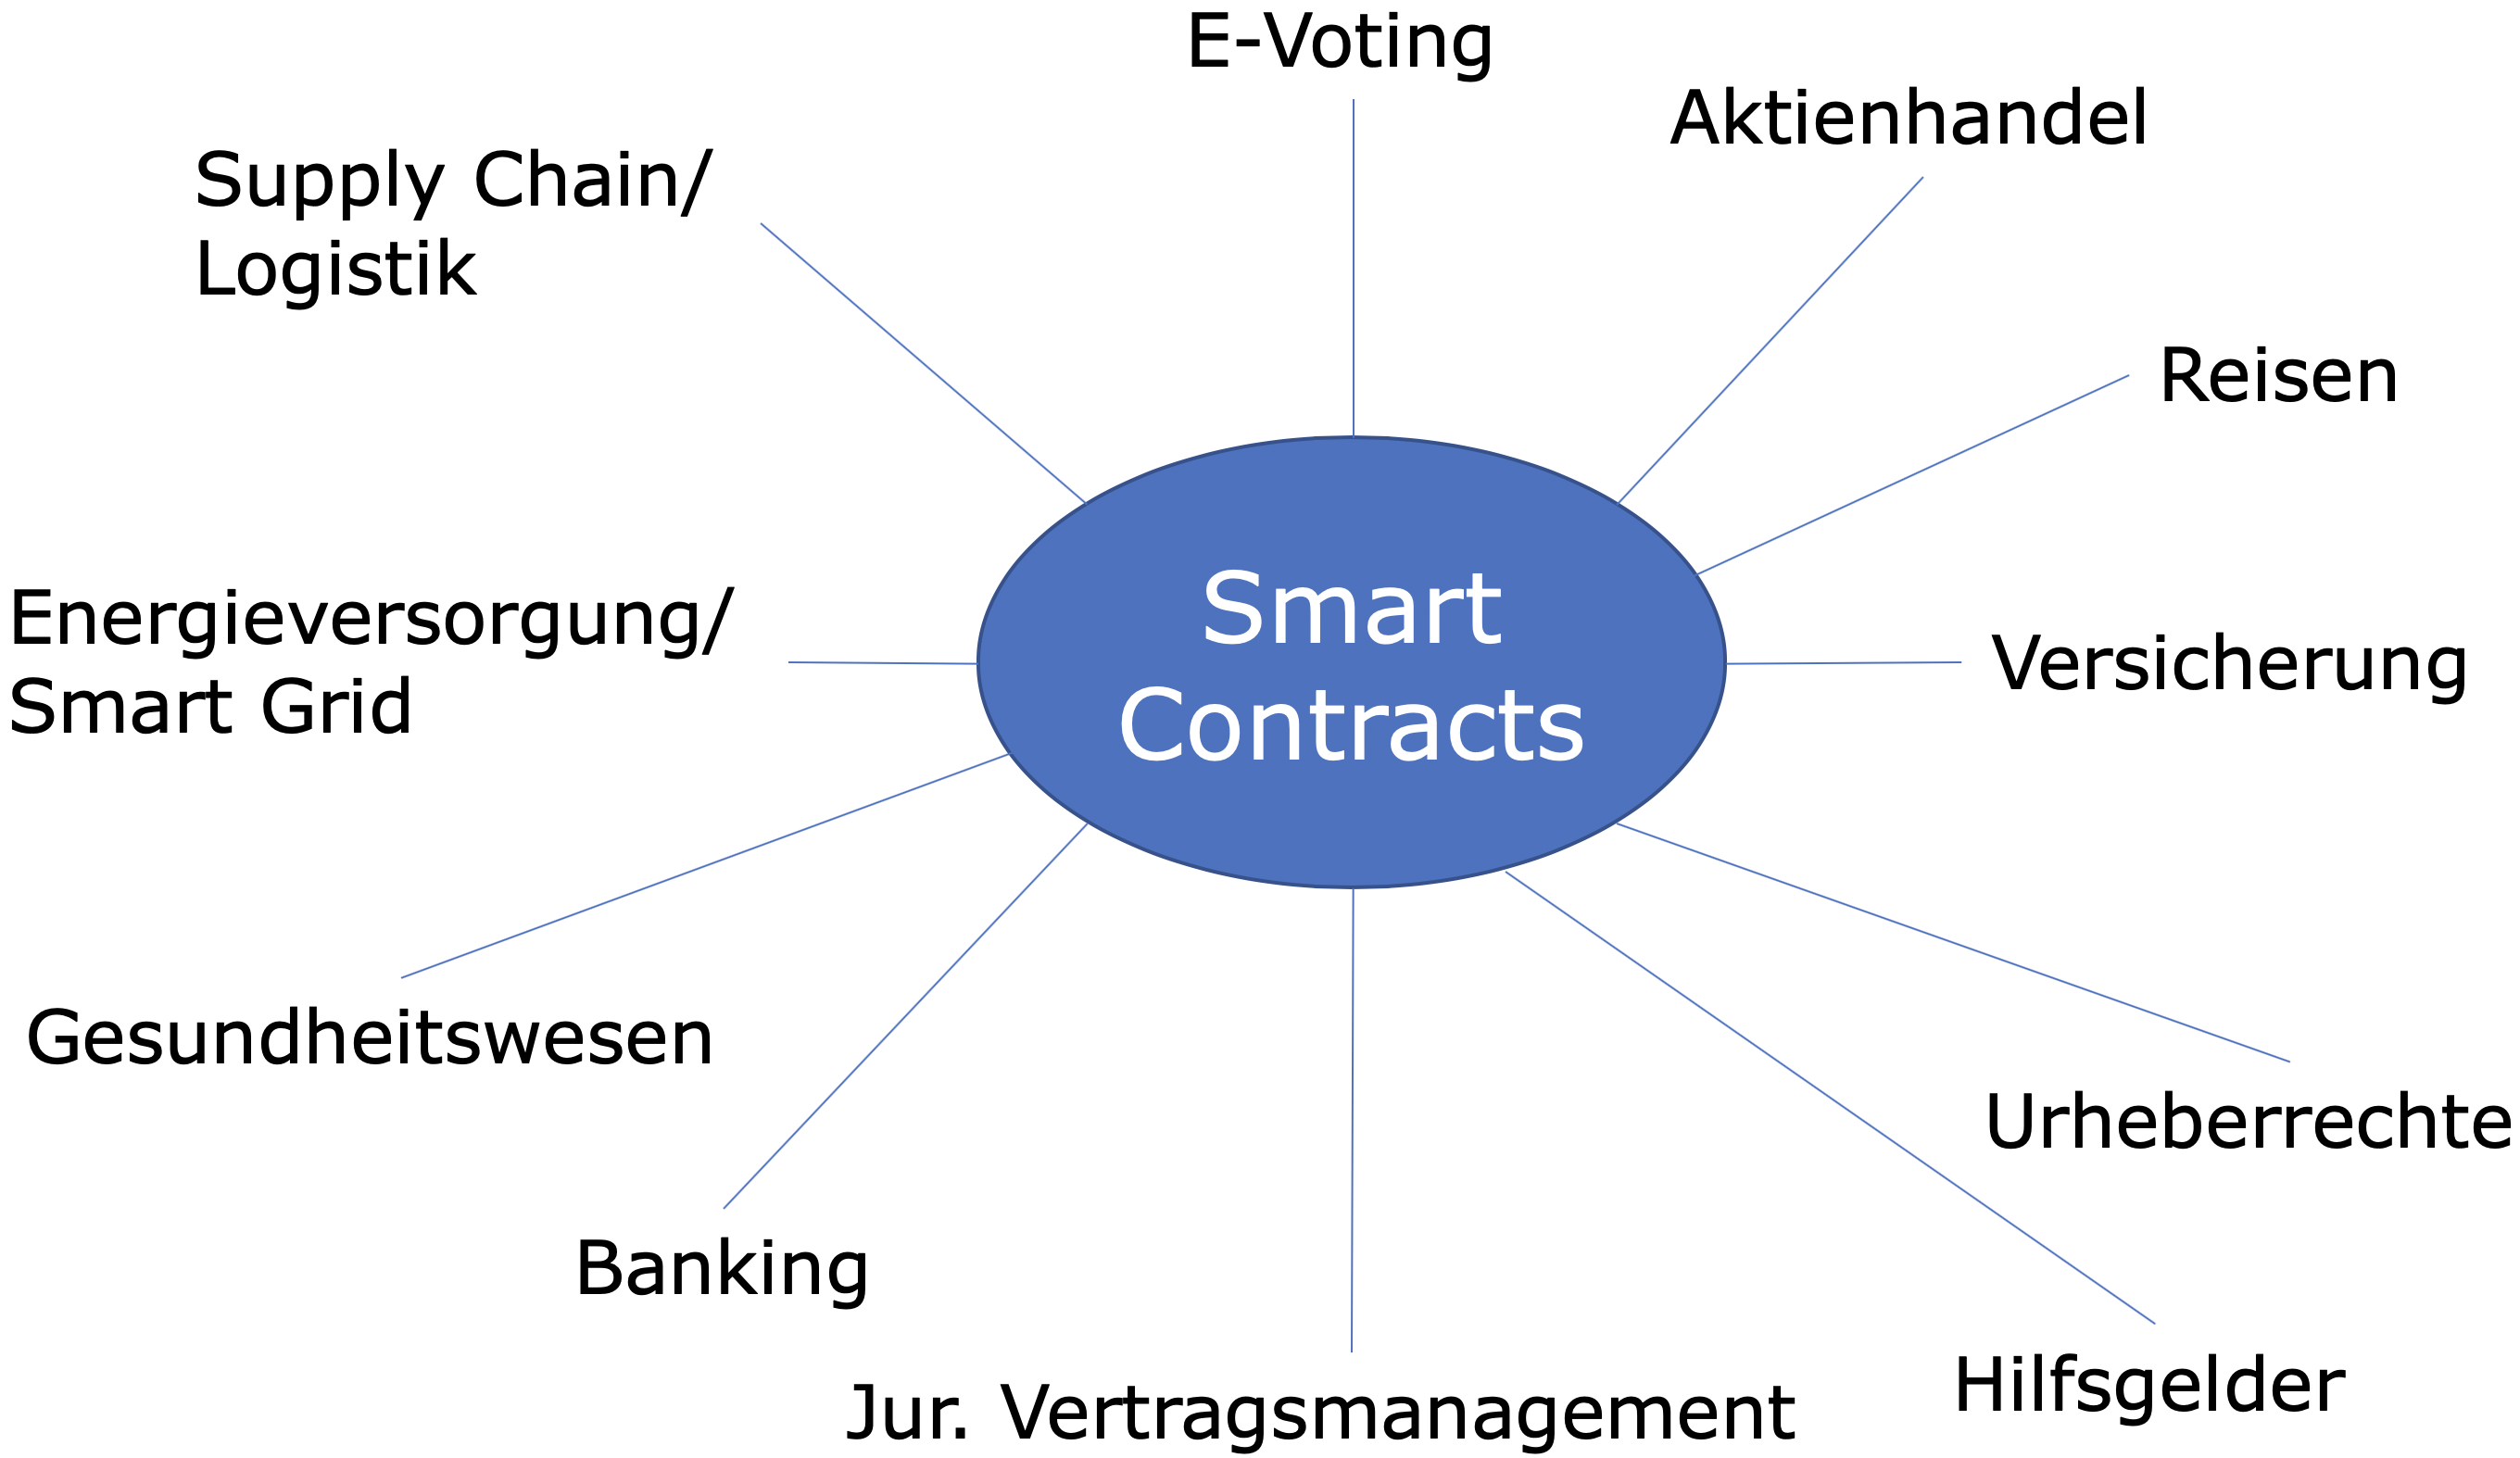
\includegraphics[width=\textwidth]{Bilder/Mindmap.png}
  \caption[Mindmap zu Smart Contracts]{Mindmap zu Smart Contracts (eigene Darstellung)}
  \label{fig:mindmap}
\end{figure}

Da es in dem geringen Umfang dieser Seminararbeit nicht möglich ist, im Detail auf alle Bereiche einzugehen, soll nun begründet dargelegt werden, wieso die jeweiligen Beispiele von der näheren Betrachtung ausgeschlossen wurden.\\ 

\textbf{E-Voting}\\
Generell ist das E-Voting ein Bereich, für den Smart Contracts prädestiniert scheinen \cite[vgl. z. B.][]{McCorry2017, Kshetri2018, Yavuz2018}. Die sichere, elektronische Abgabe von Stimmen, ist ein Thema, das viele Länder, darunter die Schweiz, beschäftigt. Diese gilt auf dem Fachgebiet seit Jahren als Pionier. Dort wurde 2018 das E-Voting in der Stadt Zug mittels Blockchain erfolgreich getestet \cite[vgl.][]{luxoft2018}. Mit Ökosystemen wie Agora wird zudem an alltagstauglichen Standards für die elektronische Stimmabgabe gearbeitet \cite[vgl.][]{Agora2019}. Trotzdem wird oftmals noch, wie in Deutschland, auf analoge Art und Weise abgestimmt. Ein Grund dafür stellt die Angreifbarkeit der Systeme dar. Daher wurde von der Schweiz die Offenlegung des Quellcodes und die Einrichtung eines Bug Bounty Programms beschlossen \cite[vgl.][]{Sperlich2019}. Überträgt man diese Gefahren auf die Blockchain, wird die Angriffsfläche durch solch eine basierte Lösung minimiert, generell sind Attacken aber nicht undurchführbar. \\
Aufgrund der allgemeinen Kontroverse über die Anwendung, sowie der Schwierigkeit, genaue Informationen über die eingesetzten Plattformen und Smart Contracts bei Blockchain-basierten Lösungen zu erhalten, wurde dieses Thema nicht zur genaueren Bearbeitung herangezogen.

\textbf{Aktienhandel}\\
Der Aktienhandel ist ein typisches Beispiel für zentralisierte Handelsplattformen. Mittels Smart Contracts und der Blockchain ließen sich an Transaktionen beteiligte Intermediäre entfernen und somit Kosten sparen \cite[vgl.][]{Notheisen2017}.\\
Eine komplett funktionierende Blockchain-Börse gibt es Stand heute nicht. Jedoch nähert sich zum Zeitpunkt des Verfassens dieser Arbeit mit SprinkleXChange die erste dieser Art ihrem Markteintritt \cite[vgl.][]{Hoikkala2019}.\\
Durch den frühen Stand der Implementierungen bzw. der Forschungskonzepte eignet sich dieses Thema nur bedingt für eine tiefe Begutachtung, weshalb es zugunsten anderer Themen nicht betrachtet wird.

\textbf{Urheberrechte}\\
Die Wahrung der Urheberrechte stellt in einer digitalen und globalisierten Welt eine große Herausforderung dar. Mit der umstrittenen EU-Reform um Artikel 13 respektive 17 sollte das Urheberrecht grundlegend erneuert werden \cite[vgl.][]{bpb2019}.\\
Musikverlage, wie Ujo Music, gehen mithilfe der Blockchain andere Wege und vertreiben über eine mehrschichtige Softwarearchitektur die Titel ihrer Künstler dezentral \cite[vgl.][]{Attar2018}. Nach ersten Tests ist die weitere Vorgehensweise jedoch unklar \cite[vgl.][S. 121 f.]{Gilli2019}.\\
Da auch hier die Entwicklungen der Industrie noch nicht absehbar und wenige konkrete Beispiele vorhanden sind, ist es nicht für diese Arbeit geeignet.

\textbf{Juristisches Vertragsmanagement}\\
Das klassische Vertragsmanagement, welches heute von einem Notar geführt wird, kann mittels Smart Contracts vereinfacht werden. Der Markt für Legal Techs, also Startups in der Rechtsbranche, scheint durchaus gegeben zu sein, da die Digitalisierung auch in diesem Bereich eine immer größere Rolle spielt. Eines davon ist die Firma TODO: [EINFÜGEN!!!!!!!!!]\\
Solange aber die rechtlichen Grundlagen für die Rechtssicherheit elektronischer Verträge in der Blockchain nicht gegeben sind, wird ihre Anwendung minimal sein.


\textbf{Banking}\\
Im Zuge der Recherche wurde der Kontakt zu Banken über öffentlich zugängliche E-Mail-Adressen gesucht. Da sich bis zum Zeitpunkt des Verfassens dieser Arbeit kein angeschriebenes Geldinstitut gemeldet hat, sind wenig verfügbare Informationen vorhanden. Allerdings zeigen Vorstöße, wie der von Wirecard \cite[vgl.][]{Weidemann2018}, dass es sich um ein durchaus interessantes Gebiet im Bankensegment handelt. Da Banken aber ohnehin darauf bedacht sein dürften, sensible Informationen wie z.B. Bankdaten nicht öffentlich zu speichern, wird in heutigen und zukünftigen Implementierungen von Smart Contracts wohl keine öffentliche Blockchain, wie beispielsweise Ethereum, herangezogen werden. \\
Das erschwert die Erlangung von Wissen über die eingesetzen Verfahren und Lösungen, weshalb Banking von den Themen ausgeschlossen wird.

\textbf{Gesundheitswesen}\\
TODO!!!

Somit verbleiben die Bereiche Reisen, Versicherung, Hilfsgelder, Energieversorgung/Smart Grid sowie Supply Chain/Logistik zur weiteren Begutachtung.